% DSM Partitioning — CPSC 482 Project Presentation
% Compile with: pdflatex presentation.tex (twice)
\documentclass[aspectratio=169]{beamer}

% ── Theme & Colours ────────────────────────────────────────────────────────────
% --- Theme Base ---
\usetheme{Madrid}
\usecolortheme{default}

% --- UNBC Brand Colors ---
\definecolor{UNBCGreen}{HTML}{004621}       % Official UNBC Dark Green
\definecolor{UNBCGold}{HTML}{FFC20E}        % Official UNBC Gold
\definecolor{UNBCLightGreen}{HTML}{2E7D4F}  % Lighter green for secondary elements
\definecolor{offwhite}{RGB}{244, 246, 249}
\definecolor{slategray}{HTML}{666666}
\definecolor{navyblue}{RGB}{28, 43, 74}  % kept for backward compat in slide body

% --- Palette (controls header/footer bar colors) ---
\setbeamercolor{palette primary}{bg=UNBCGreen, fg=white}
\setbeamercolor{palette secondary}{bg=UNBCLightGreen, fg=white}
\setbeamercolor{palette tertiary}{bg=UNBCGreen, fg=white}
\setbeamercolor{palette quaternary}{bg=UNBCGreen, fg=white}

% --- Structure & Titles ---
\setbeamercolor{structure}{fg=UNBCGreen}
\setbeamercolor{frametitle}{bg=UNBCGreen, fg=white}
\setbeamercolor{title}{fg=white}
\setbeamercolor{subtitle}{fg=UNBCGold}
\setbeamercolor{section title}{fg=UNBCGreen}

% --- Blocks ---
\setbeamercolor{block title}{bg=UNBCGreen, fg=white}
\setbeamercolor{block body}{bg=offwhite, fg=black}
\setbeamercolor{block title alerted}{bg=UNBCGold, fg=black}  % Gold alerted block
\setbeamercolor{block body alerted}{bg=offwhite, fg=black}

% --- Lists ---
\setbeamercolor{itemize item}{fg=UNBCGreen}
\setbeamercolor{itemize subitem}{fg=UNBCGold}

% --- Progress Bar (if using a theme that supports it) ---
\setbeamercolor{progress bar}{fg=UNBCGold, bg=gray!30}

% --- Remove default nav symbols ---
\setbeamertemplate{navigation symbols}{}

% --- Custom Footline ---
\setbeamertemplate{footline}{%
  \leavevmode%
  \hbox{%
    \begin{beamercolorbox}[wd=.33\paperwidth,ht=2.25ex,dp=1ex,center]{palette secondary}%
      \usebeamerfont{author in head/foot}Kraft, Payne, Sall
    \end{beamercolorbox}%
    \begin{beamercolorbox}[wd=.34\paperwidth,ht=2.25ex,dp=1ex,center]{palette primary}%
      \usebeamerfont{title in head/foot}DSM Partitioning — CPSC 482
    \end{beamercolorbox}%
    \begin{beamercolorbox}[wd=.33\paperwidth,ht=2.25ex,dp=1ex,right]{palette quaternary}%
      \usebeamerfont{date in head/foot}\insertshortdate{}\hspace*{1em}%
      \insertframenumber{} / \inserttotalframenumber\hspace*{1ex}
    \end{beamercolorbox}%
  }%
}

% ── Packages ──────────────────────────────────────────────────────────────────
\usepackage[utf8]{inputenc}
\usepackage[T1]{fontenc}
\usepackage{amsmath,amssymb}
\usepackage{booktabs}
\usepackage{graphicx}
\usepackage{tikz}
\usetikzlibrary{arrows.meta, positioning, shapes.geometric}
\usepackage{algorithm}
\usepackage{algpseudocode}

% ── Title info ─────────────────────────────────────────────────────────────────
\title[DSM Partitioning]{DSM Partitioning}
\subtitle{A Pipeline for Reordering \\ Dependency Structure Matrices}
\author[Kraft, Payne, El Sall]{Simon Kraft \and Joshua Payne \and El Sall}
\institute[UNBC]{CPSC 482/682 — Data Structures II\\University of Northern British Columbia}
\date{April 7, 2026}

% ── Helper command ────────────────────────────────────────────────────────────
\newcommand{\highlight}[1]{\textcolor{teal}{\textbf{#1}}}
\newcommand{\alertword}[1]{\textcolor{orange}{\textbf{#1}}}

% ══════════════════════════════════════════════════════════════════════════════
\begin{document}

% ── Title Slide ───────────────────────────────────────────────────────────────
\begin{frame}
  \titlepage
\end{frame}

% ── Outline ───────────────────────────────────────────────────────────────────
\begin{frame}{Outline}
  \tableofcontents
\end{frame}

% ══════════════════════════════════════════════════════════════════════════════
\section{Introduction}
% ══════════════════════════════════════════════════════════════════════════════

\begin{frame}{Motivation}
  \begin{columns}[T]
    \begin{column}{0.48\textwidth}
      \textbf{The challenge:}
      \begin{itemize}
        \item Modern software \& engineering projects involve \highlight{hundreds to thousands of interdependent tasks} across diverse teams
        \item Traditional tools (Gantt, CPM) handle sequential \& parallel flows well\ldots
        \item \ldots but \alertword{fail for interdependent tasks} where outputs feed back as inputs
        \item These feedback dependencies are common in complex product development
      \end{itemize}
    \end{column}
    \begin{column}{0.48\textwidth}
      \begin{block}{Goal}
        Find a \textbf{task ordering} that minimises conflicts in information flow to enable faster, more predictable project execution.
      \end{block}
      \vspace{0.5em}
      \begin{alertblock}{Key observation}
        When task~$j$ supplies input to task~$i$ but is scheduled \emph{after} it, assumptions must
        be made. If wrong, task~$i$ must be \textbf{re-executed}.
      \end{alertblock}
    \end{column}
  \end{columns}
\end{frame}

\begin{frame}{Design Structure Matrix (DSM)}
  \begin{columns}[T]
    \begin{column}{0.5\textwidth}
      \textbf{Definition:} A binary matrix $A \in \{0,1\}^{n\times n}$ where
      \[
        a_{ij} = 1 \iff \text{task } i \text{ depends on task } j
      \]
      \begin{itemize}
        \item Rows and columns labeled by the same task list
        \item Diagonal entries carry no dependency information.
        \item Equivalent to directed graph $G(A) = (V,E)$
      \end{itemize}
      \vspace{0.4em}
    \end{column}
    \begin{column}{0.46\textwidth}
      \begin{block}{Three dependency types:}
        \begin{itemize}
          \item \highlight{Feed-Forward} ($j < i$): below diagonal — easy
          \item \alertword{Feed-Back} ($j > i$): above diagonal — problematic
          \item \textcolor{red}{Coupled}: mutual dependency — hardest
        \end{itemize}
      \end{block}
    \end{column}
  \end{columns}
\end{frame}


\begin{frame}{The Partitioning Problem}
  \textbf{Objective:} Find $P \in \{0,1\}^{n\times n}$ such that $A' = P^\top A P$ minimises:
  \vspace{0.3em}
  \begin{columns}[T]
    \begin{column}{0.48\textwidth}
      \begin{block}{Objective 1 — Feed-Back Marks}
        \[
          |\text{FBM}| = \bigl|\{a'_{ij} \neq 0 \mid j > i\}\bigr|
        \]
        Minimise the \textbf{count} of above-diagonal nonzeros.
      \end{block}
    \end{column}
    \begin{column}{0.48\textwidth}
      \begin{block}{Objective 2 — Feedback Distance}
        \[
          \text{TFBD} = \sum_{a'_{ij} \in \text{FBM}} (j - i)
        \]
        Minimise the \textbf{distance} of feed-back marks from the diagonal.
      \end{block}
    \end{column}
  \end{columns}
  \vspace{0.5em}
  \begin{columns}[T]
    \begin{column}{0.48\textwidth}
      \begin{alertblock}{Best case}
        $G(A)$ has no directed cycles $\Rightarrow$ fully lower triangular,\\$|\text{FBM}| = 0$, $\text{TFBD} = 0$
      \end{alertblock}
    \end{column}
    \begin{column}{0.48\textwidth}
      \begin{alertblock}{General case}
        Achieve \highlight{Block Lower Triangular Form (BLTF)}: group mutually dependent tasks into diagonal blocks and push remaining feed-back marks close to the diagonal.
      \end{alertblock}
    \end{column}
  \end{columns}
\end{frame}

% ══════════════════════════════════════════════════════════════════════════════
\section{Methodology}
% ══════════════════════════════════════════════════════════════════════════════

\begin{frame}{Our 6-Stage Pipeline}
  \centering
  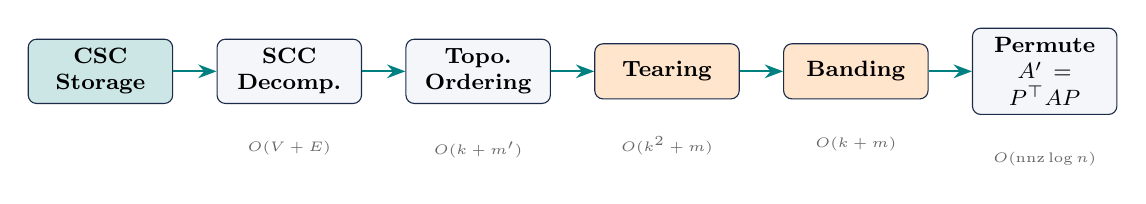
\begin{tikzpicture}[
    node distance=0.55cm,
    box/.style={rectangle, rounded corners=3pt, draw=navyblue, fill=offwhite,
                text width=1.6cm, align=center, font=\footnotesize\bfseries, minimum height=0.7cm},
    arr/.style={-Stealth, thick, color=teal}
  ]
    \node[box, fill=teal!20] (csc)  {CSC\\Storage};
    \node[box, right=of csc] (scc)  {SCC\\Decomp.};
    \node[box, right=of scc] (topo) {Topo.\\Ordering};
    \node[box, right=of topo, fill=orange!20] (tear) {Tearing};
    \node[box, right=of tear, fill=orange!20] (band) {Banding};
    \node[box, right=of band] (perm) {Permute\\$A' = P^\top AP$};

    \draw[arr] (csc)  -- (scc);
    \draw[arr] (scc)  -- (topo);
    \draw[arr] (topo) -- (tear);
    \draw[arr] (tear) -- (band);
    \draw[arr] (band) -- (perm);

    \node[below=0.35cm of scc,  font=\tiny, color=slategray] {$O(V+E)$};
    \node[below=0.35cm of topo, font=\tiny, color=slategray] {$O(k+m')$};
    \node[below=0.35cm of tear, font=\tiny, color=slategray] {$O(k^2+m)$};
    \node[below=0.35cm of band, font=\tiny, color=slategray] {$O(k+m)$};
    \node[below=0.35cm of perm, font=\tiny, color=slategray] {$O(\text{nnz}\log n)$};
  \end{tikzpicture}

  \vspace{0.6em}
  \begin{columns}[T]
    \begin{column}{0.48\textwidth}
      \begin{block}{Data Structure: CSC}
        \begin{itemize}
          \item Column pointer array \texttt{col\_ptr}$[0\ldots n]$
          \item Row index array \texttt{row\_ind}$[0\ldots\text{nnz}-1]$
          \item Storage: $\Theta(n + \text{nnz})$
          \item No value array needed (binary DSM)
        \end{itemize}
      \end{block}
    \end{column}
    \begin{column}{0.48\textwidth}
      \begin{block}{Why CSC?}
        Column $j$ gives the neighbours of vertex $j$\\
        in $O(\deg(j))$ — ideal for DFS traversal.
      \end{block}
    \end{column}
  \end{columns}
\end{frame}

\begin{frame}{SCC Decomposition}
  Both algorithms built on a shared iterative DFS with callback hooks, using an explicit stack (no recursion). 

  \vspace{0.4em}
  \begin{columns}[T]
    \begin{column}{0.48\textwidth}
      \begin{block}{Tarjan's Algorithm}
        \begin{itemize}
          \item \textbf{Single DFS pass}
          \item Each vertex $v$ maintains $\mathit{low}(v)$: smallest reachable pre-order time
          \item $\mathit{low}(v) = v.\mathit{pre}$ at finish $\Rightarrow$ $v$ is SCC root; pop stack
          \item $O(V+E)$ time, $O(V)$ space
        \end{itemize}
      \end{block}
    \end{column}
    \begin{column}{0.48\textwidth}
      \begin{block}{Kosaraju-Sharir Algorithm}
        \begin{itemize}
          \item \textbf{Two DFS passes}
          \item Pass 1: DFS on $G$, record finish order
          \item Pass 2: DFS on $\mathit{rev}(G)$ in reverse finish order; each DFS tree = one SCC
          \item $O(V+E)$ time, $O(V+E)$ space
        \end{itemize}
      \end{block}
    \end{column}
  \end{columns}

  \vspace{0.4em}
  After SCC decomposition, the \highlight{condensation DAG} is topologically sorted with
  \textbf{Kahn's algorithm} to determine the block ordering.
\end{frame}

\begin{frame}{Tearing \& Banding}
  \begin{columns}[T]
    \begin{column}{0.48\textwidth}
      \begin{block}{Tearing (reduces FBM within SCCs)}
        \begin{itemize}
          \item \textbf{Algorithm~GR} (Eades, Lin, Smyth):
          \item Repeatedly peel sinks $\to$ append to back, sources $\to$ prepend to front
          \item When neither exists, pick vertex with max $d^+ - d^-$ as a source
          \item The resulting ordering defines which edges are feedback arcs (backward edges)
        \end{itemize}
      \end{block}
    \end{column}
    \begin{column}{0.48\textwidth}
      \begin{block}{Banding (reduces TFBD within SCCs)}
        \begin{itemize}
          \item \textbf{Reverse Cuthill-McKee (RCM)}: concentrates nonzeros near diagonal
          \item \textbf{Adjacent-swap refinement}: accepts swaps that lower TFBD without increasing FBM
          \item Best of torn + RCM orderings kept
        \end{itemize}
      \end{block}
    \end{column}
  \end{columns}
\end{frame}

\begin{frame}{Experimental Setup}
  \begin{block}{Benchmark suite}
    \begin{itemize}
      \item 10 sparse matrices from the project repository
      \item Dimensions: $n = 11$ to $27{,}770$, nnz $= 4$ to $352{,}807$
    \end{itemize}
  \end{block}
  \vspace{0.5em}
  \begin{block}{Hardware \& methodology}
    \begin{itemize}
      \item Apple M2 / 8\,GB RAM (L1d 64\,KB, L1i 128\,KB, L2 4\,MB), compiled with \texttt{-O3}, Apple LLVM 17
      \item Each algorithm: 2 warm-up + 5 timed runs
      \item Metrics: FBM count, TFBD, and mean runtime ($\mu$s)
    \end{itemize}
  \end{block}
\end{frame}

% ══════════════════════════════════════════════════════════════════════════════
\section{Results}
% ══════════════════════════════════════════════════════════════════════════════

\begin{frame}{Stage-wise Quality Improvement}
  \begin{columns}[T]
    \begin{column}{0.52\textwidth}
      \textbf{Average reductions across 10 matrices:}
      \vspace{0.3em}
      \begin{tabular}{lcc}
        \toprule
        Stage & FBM $\downarrow$ & TFBD $\downarrow$ \\
        \midrule
        Baseline       & ---      & ---     \\
        TopoOnly       & 60.16\%  & 86.56\% \\
        + Tearing      & 76.47\%  & \textit{slight} $\uparrow$ \\
        + Banding      & \highlight{76.50\%}  & \highlight{85.95\%} \\
        \bottomrule
      \end{tabular}
      \vspace{0.5em}
      \begin{itemize}
        \item Topo ordering provides the \textbf{largest single gain}
        \item Tearing drives further FBM reduction within SCCs
        \item Banding polishes TFBD without hurting FBM
      \end{itemize}
    \end{column}
    \begin{column}{0.44\textwidth}
      \begin{block}{Selected matrix results}
        \small
        \begin{tabular}{lrr}
          \toprule
          Matrix & FBM$_0 \to$ FBM$_f$ & TFBD$_f$ \\
          \midrule
          Tina\_AskCal & $12 \to 4$       & 7 \\
          California   & $6063 \to 192$   & 669 \\
          wb-cs-stanford & $20131 \to 8537$ & 1.78M \\
          HEP-th-new   & $104435 \to 8281$ & 10.1M \\
          \bottomrule
        \end{tabular}
      \end{block}
    \end{column}
  \end{columns}
\end{frame}


\begin{frame}{FBM Reduction}
  \begin{figure}
    \centering
    
\includegraphics[width=0.85\textwidth]{../out/plots/optimization_fbm_reduction.png}
  \end{figure}
\end{frame}

\begin{frame}{TFBD Reduction}
  \begin{figure}
    \centering
    \includegraphics[width=0.85\textwidth]{../out/plots/optimization_tfbd_reduction.png}
  \end{figure}
\end{frame}

\begin{frame}{Runtime Comparison: Tarjan vs.\ Kosaraju-Sharir}
  \begin{columns}[T]
    \begin{column}{0.48\textwidth}
      \begin{block}{Key findings}
        \begin{itemize}
          \item Both algorithms produce \textbf{identical SCC decompositions}
          \item Tarjan: mean $\approx 560\,\mu$s
          \item Kosaraju-Sharir: mean $\approx 992\,\mu$s
          \item Tarjan is $\approx \mathbf{1.77\times}$ faster on average
          \item Scaling compatible with expected $O(V+E)$ near-linear behaviour
        \end{itemize}
      \end{block}
      \vspace{0.3em}
      \begin{alertblock}{Why is Tarjan faster?}
        Single DFS pass vs.\ two passes + transpose graph construction in Kosaraju-Sharir.
      \end{alertblock}
    \end{column}
    \begin{column}{0.48\textwidth}
      \begin{block}{Pipeline stage runtimes}
        \small
        \begin{tabular}{lr}
          \toprule
          Stage & Relative cost \\
          \midrule
          Tarjan SCC    & low \\
          Kosaraju SCC  & $1.77\times$ Tarjan \\
          Condensation  & low \\
          Topo sort     & low \\
          Tearing       & moderate \\
          Banding       & highest \\
          Permutation   & low \\
          \bottomrule
        \end{tabular}
      \end{block}
    \end{column}
  \end{columns}
\end{frame}

\begin{frame}{Runtime Comparison: Pipeline}
  \begin{figure}
    \centering
    
\includegraphics[width=0.75\textwidth]{../out/plots/scaling.png}
  \end{figure}
\end{frame}

\begin{frame}{Qualitative Results: California}
  \begin{figure}
    \centering
    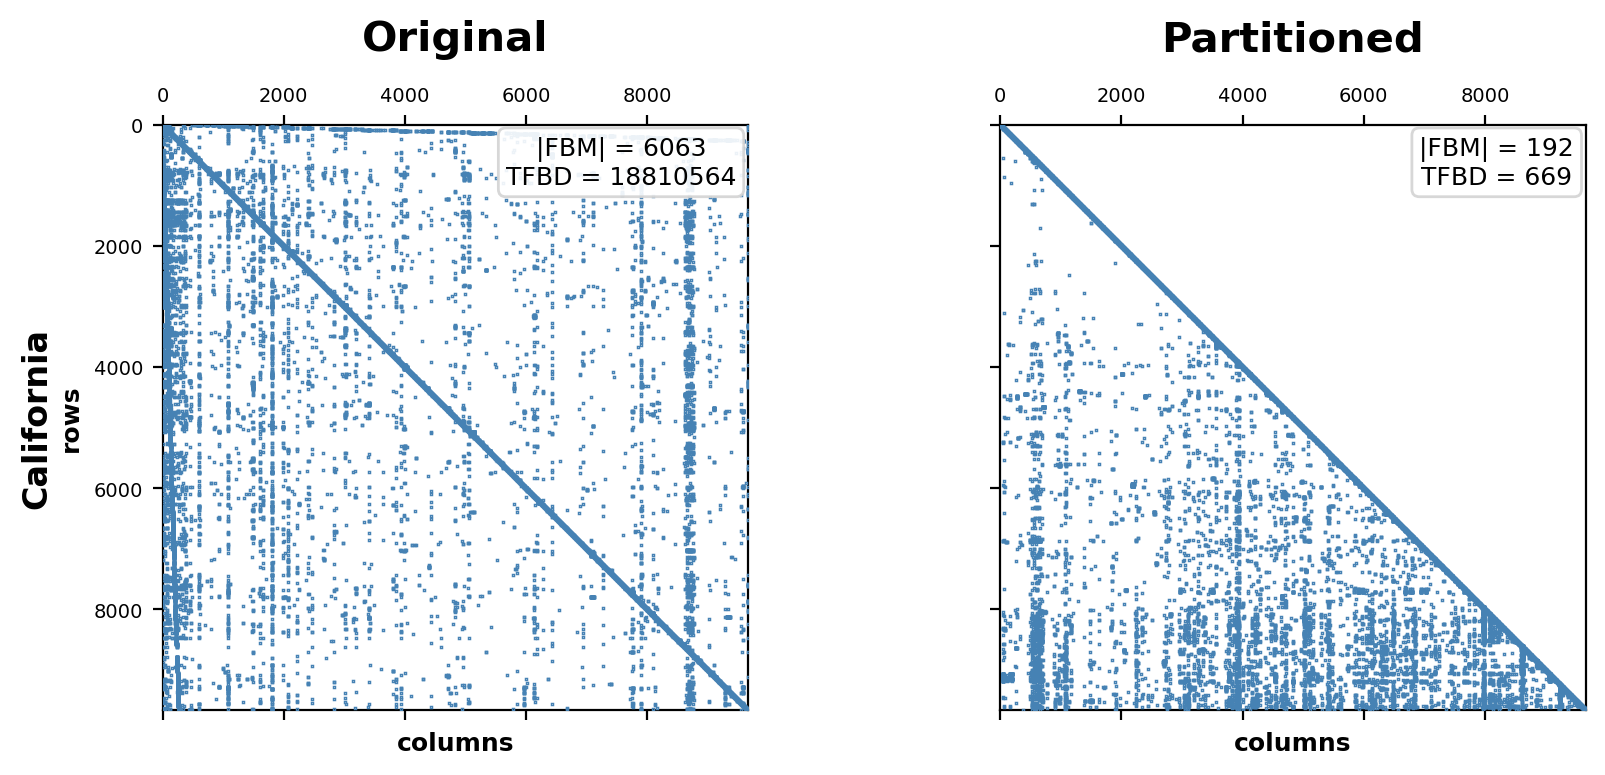
\includegraphics[width=0.9\textwidth]{figures/California.png}
  \end{figure}
\end{frame}

\begin{frame}{Qualitative Results: GD99\_c}
  \begin{figure}
    \centering
    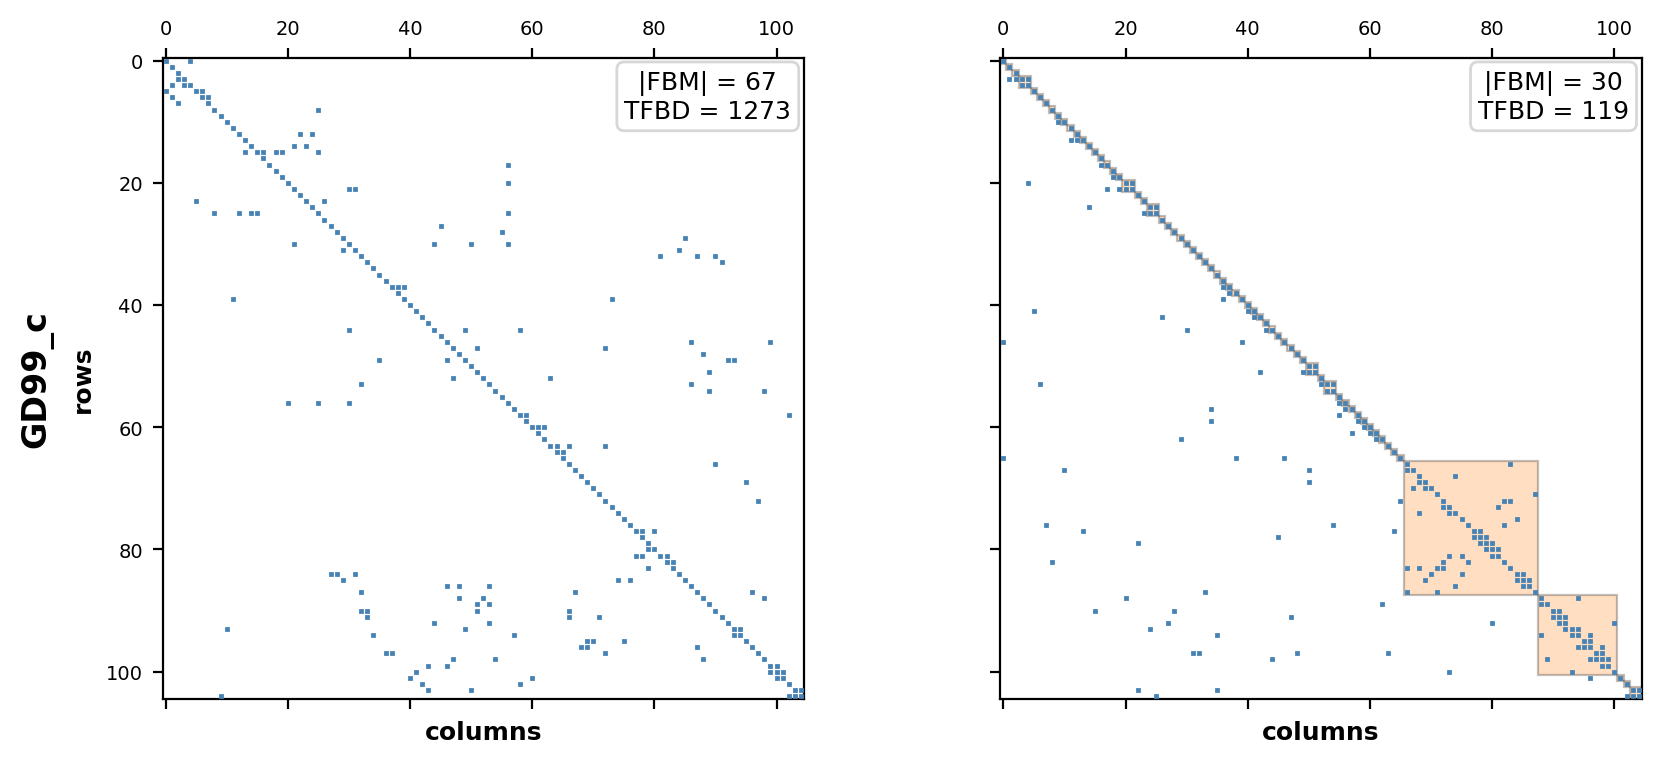
\includegraphics[width=0.9\textwidth]{figures/GD99_c.png}
  \end{figure}
\end{frame}

\begin{frame}{Qualitative Results: wb-cs-stanford}
  \begin{figure}
    \centering
    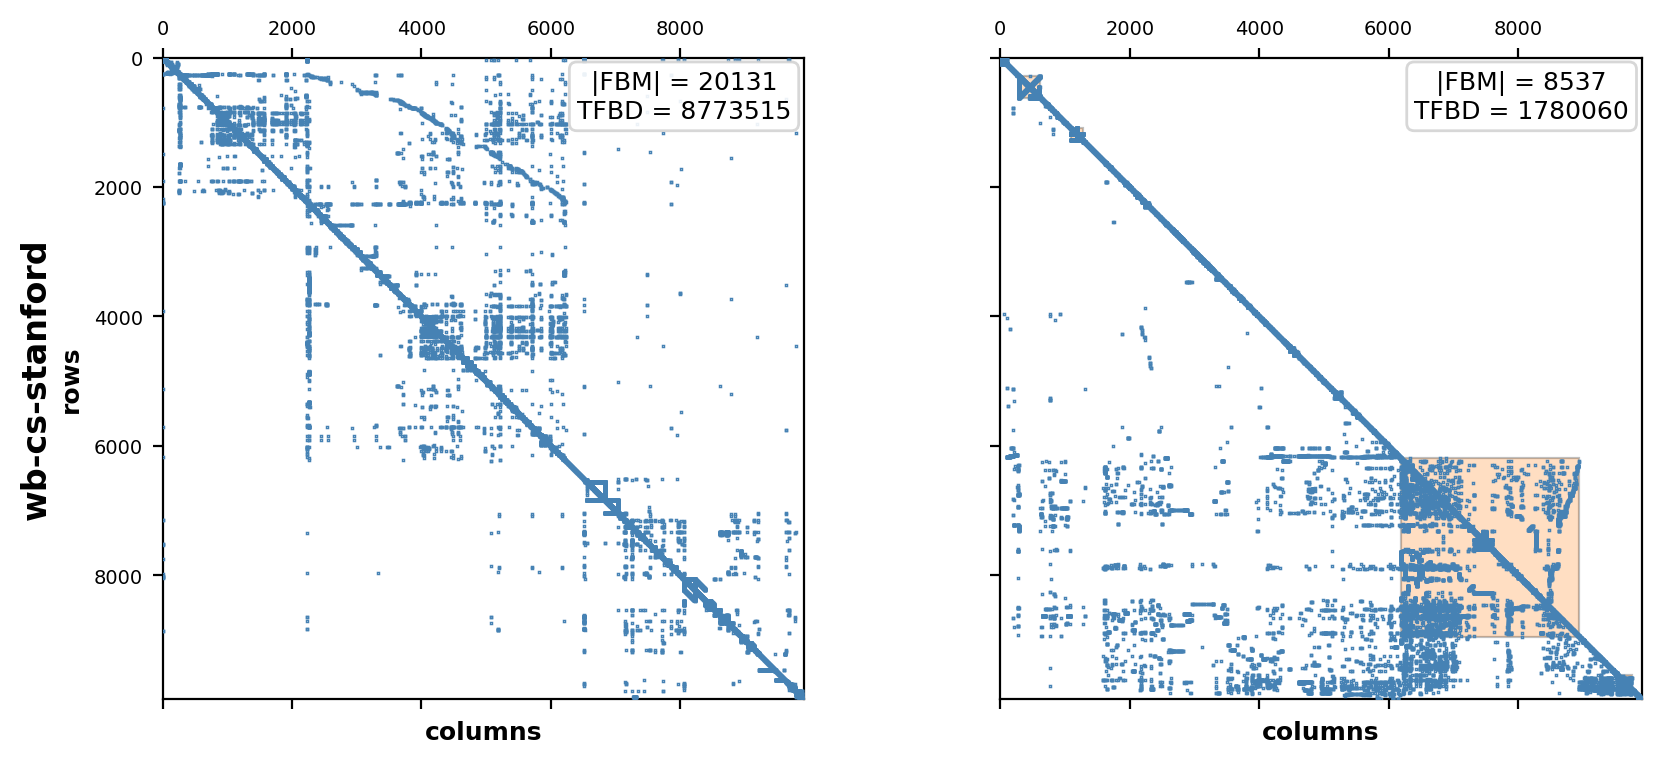
\includegraphics[width=0.9\textwidth]{figures/wb-cs-stanford.png}
  \end{figure}
\end{frame}

% ══════════════════════════════════════════════════════════════════════════════
\section{Conclusions}
% ══════════════════════════════════════════════════════════════════════════════

\begin{frame}{Conclusions \& Future Work}
  \begin{columns}[T]
    \begin{column}{0.48\textwidth}
      \begin{block}{What we achieved}
        \begin{itemize}
          \item Implemented full 6-stage DSM reordering pipeline in C++ with CSC
          \item Both Tarjan and Kosaraju-Sharir SCC algorithms — identical decompositions
          \item \highlight{76.50\% average FBM reduction}, \highlight{85.95\% average TFBD reduction} across 10 benchmark matrices
          \item Tarjan $1.77\times$ faster than Kosaraju-Sharir
          \item Runtime scales near-linearly with $V + E$
        \end{itemize}
      \end{block}
    \end{column}
    \begin{column}{0.48\textwidth}
      \begin{block}{Future directions}
        \begin{itemize}
          \item \textbf{Better tearing}: replace greedy Algorithm~GR with an exact or improved heuristic for minimum feedback arc set
          \item \textbf{Parallelism}: per-SCC tearing \& banding are independent — parallelise for large matrices
          \item \textbf{Weighted DSMs}: extend to numerical dependency strengths; optimise weighted feedback cost
        \end{itemize}
      \end{block}
    \end{column}
  \end{columns}
\end{frame}

% ══════════════════════════════════════════════════════════════════════════════
\section*{Acknowledgements \& Team Contribution}
% ══════════════════════════════════════════════════════════════════════════════

\begin{frame}{Acknowledgements \& Team Contributions}
  \begin{block}{AI Disclosure}
    Claude (Anthropic) and ChatGPT (OpenAI) were used to aid understanding of concepts and sourcing literature. 
  \end{block}

  \vspace{0.5em}
  \begin{block}{Team Member Contributions}
    \begin{tabular}{l p{0.72\textwidth}}
      \toprule
      \textbf{Member} & \textbf{Contribution} \\
      \midrule
      Simon Kraft   & Implemented Tarjan's algorithm, Topological Sort. Wrote report introduction and abstract. \\
      Joshua Payne  & Implemented Kosaraju-Sharir algorithm, tearing \& banding. Wrote report description of solution. \\
      El Sall       & Implemented Permutation application and benchmark suite. Wrote report numerical results section. \\
      \bottomrule
    \end{tabular}
  \end{block}

  \vspace{0.3em}
  \centering
  \large \textbf{Thank you — questions welcome!}
\end{frame}

\end{document}
